% Sketch output, version 0.2 (build 161, Tue Sep 8 23:35:27 2009)
% Output language: PGF/TikZ,LaTeX
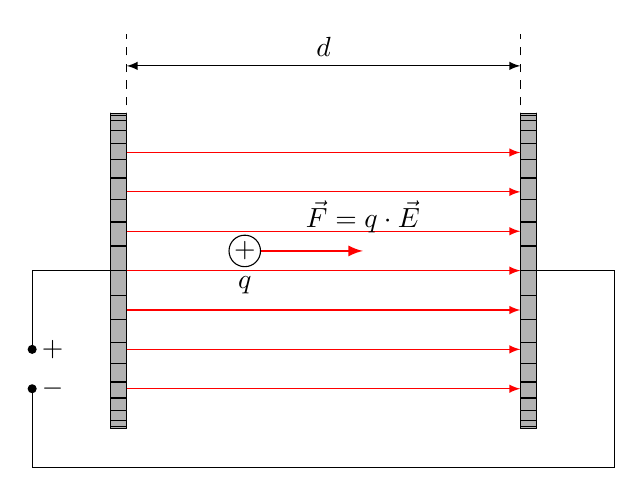
\begin{tikzpicture}[line join=round]
\filldraw[fill=gray!30](-.2,2)--(-.2,1.975)--(-.2,1.902)--(-.2,1.782)--(-.2,1.618)--(-.2,1.414)--(-.2,1.176)--(-.2,.908)--(-.2,.618)--(-.2,.313)--(-.2,0)--(-.2,-.313)--(-.2,-.618)--(-.2,-.908)--(-.2,-1.176)--(-.2,-1.414)--(-.2,-1.618)--(-.2,-1.782)--(-.2,-1.902)--(-.2,-1.975)--(-.2,-2)--(-.2,-1.975)--(-.2,-1.902)--(-.2,-1.782)--(-.2,-1.618)--(-.2,-1.414)--(-.2,-1.176)--(-.2,-.908)--(-.2,-.618)--(-.2,-.313)--(-.2,0)--(-.2,.313)--(-.2,.618)--(-.2,.908)--(-.2,1.176)--(-.2,1.414)--(-.2,1.618)--(-.2,1.782)--(-.2,1.902)--(-.2,1.975)--cycle;
\filldraw[fill=gray!30](0,1.975)--(0,1.902)--(0,1.782)--(0,1.618)--(0,1.414)--(0,1.176)--(0,.908)--(0,.618)--(0,.313)--(0,0)--(0,-.313)--(0,-.618)--(0,-.908)--(0,-1.176)--(0,-1.414)--(0,-1.618)--(0,-1.782)--(0,-1.902)--(0,-1.975)--(0,-2)--(0,-1.975)--(0,-1.902)--(0,-1.782)--(0,-1.618)--(0,-1.414)--(0,-1.176)--(0,-.908)--(0,-.618)--(0,-.313)--(0,0)--(0,.313)--(0,.618)--(0,.908)--(0,1.176)--(0,1.414)--(0,1.618)--(0,1.782)--(0,1.902)--(0,1.975)--(0,2)--cycle;
\filldraw[fill=gray!30](5.2,1.975)--(5.2,1.902)--(5.2,1.782)--(5.2,1.618)--(5.2,1.414)--(5.2,1.176)--(5.2,.908)--(5.2,.618)--(5.2,.313)--(5.2,0)--(5.2,-.313)--(5.2,-.618)--(5.2,-.908)--(5.2,-1.176)--(5.2,-1.414)--(5.2,-1.618)--(5.2,-1.782)--(5.2,-1.902)--(5.2,-1.975)--(5.2,-2)--(5.2,-1.975)--(5.2,-1.902)--(5.2,-1.782)--(5.2,-1.618)--(5.2,-1.414)--(5.2,-1.176)--(5.2,-.908)--(5.2,-.618)--(5.2,-.313)--(5.2,0)--(5.2,.313)--(5.2,.618)--(5.2,.908)--(5.2,1.176)--(5.2,1.414)--(5.2,1.618)--(5.2,1.782)--(5.2,1.902)--(5.2,1.975)--(5.2,2)--cycle;
\filldraw[fill=gray!30](5,2)--(5,1.975)--(5,1.902)--(5,1.782)--(5,1.618)--(5,1.414)--(5,1.176)--(5,.908)--(5,.618)--(5,.313)--(5,0)--(5,-.313)--(5,-.618)--(5,-.908)--(5,-1.176)--(5,-1.414)--(5,-1.618)--(5,-1.782)--(5,-1.902)--(5,-1.975)--(5,-2)--(5,-1.975)--(5,-1.902)--(5,-1.782)--(5,-1.618)--(5,-1.414)--(5,-1.176)--(5,-.908)--(5,-.618)--(5,-.313)--(5,0)--(5,.313)--(5,.618)--(5,.908)--(5,1.176)--(5,1.414)--(5,1.618)--(5,1.782)--(5,1.902)--(5,1.975)--cycle;
\filldraw[fill=gray!60](5,1.975)--(5.2,1.975)--(5.2,2)--(5,2)--cycle;
\filldraw[fill=gray!60](-.2,1.975)--(0,1.975)--(0,2)--(-.2,2)--cycle;
\filldraw[fill=gray!60](-.2,-2)--(0,-2)--(0,-1.975)--(-.2,-1.975)--cycle;
\filldraw[fill=gray!60](5,-2)--(5.2,-2)--(5.2,-1.975)--(5,-1.975)--cycle;
\filldraw[fill=gray!60](5,1.902)--(5.2,1.902)--(5.2,1.975)--(5,1.975)--cycle;
\filldraw[fill=gray!60](-.2,1.902)--(0,1.902)--(0,1.975)--(-.2,1.975)--cycle;
\filldraw[fill=gray!60](-.2,-1.975)--(0,-1.975)--(0,-1.902)--(-.2,-1.902)--cycle;
\filldraw[fill=gray!60](5,-1.975)--(5.2,-1.975)--(5.2,-1.902)--(5,-1.902)--cycle;
\filldraw[fill=gray!60](5,1.782)--(5.2,1.782)--(5.2,1.902)--(5,1.902)--cycle;
\filldraw[fill=gray!60](-.2,1.782)--(0,1.782)--(0,1.902)--(-.2,1.902)--cycle;
\filldraw[fill=gray!60](-.2,-1.902)--(0,-1.902)--(0,-1.782)--(-.2,-1.782)--cycle;
\filldraw[fill=gray!60](5,-1.902)--(5.2,-1.902)--(5.2,-1.782)--(5,-1.782)--cycle;
\filldraw[fill=gray!60](5,1.618)--(5.2,1.618)--(5.2,1.782)--(5,1.782)--cycle;
\filldraw[fill=gray!60](-.2,1.618)--(0,1.618)--(0,1.782)--(-.2,1.782)--cycle;
\filldraw[fill=gray!60](-.2,-1.782)--(0,-1.782)--(0,-1.618)--(-.2,-1.618)--cycle;
\filldraw[fill=gray!60](5,-1.782)--(5.2,-1.782)--(5.2,-1.618)--(5,-1.618)--cycle;
\filldraw[fill=gray!60](5,1.414)--(5.2,1.414)--(5.2,1.618)--(5,1.618)--cycle;
\filldraw[fill=gray!60](-.2,1.414)--(0,1.414)--(0,1.618)--(-.2,1.618)--cycle;
\filldraw[fill=gray!60](-.2,-1.618)--(0,-1.618)--(0,-1.414)--(-.2,-1.414)--cycle;
\filldraw[fill=gray!60](5,-1.618)--(5.2,-1.618)--(5.2,-1.414)--(5,-1.414)--cycle;
\filldraw[fill=gray!60](5,1.176)--(5.2,1.176)--(5.2,1.414)--(5,1.414)--cycle;
\filldraw[fill=gray!60](-.2,1.176)--(0,1.176)--(0,1.414)--(-.2,1.414)--cycle;
\filldraw[fill=gray!60](-.2,-1.414)--(0,-1.414)--(0,-1.176)--(-.2,-1.176)--cycle;
\filldraw[fill=gray!60](5,-1.414)--(5.2,-1.414)--(5.2,-1.176)--(5,-1.176)--cycle;
\filldraw[fill=gray!60](5,.908)--(5.2,.908)--(5.2,1.176)--(5,1.176)--cycle;
\filldraw[fill=gray!60](-.2,.908)--(0,.908)--(0,1.176)--(-.2,1.176)--cycle;
\filldraw[fill=gray!60](-.2,-1.176)--(0,-1.176)--(0,-.908)--(-.2,-.908)--cycle;
\filldraw[fill=gray!60](5,-1.176)--(5.2,-1.176)--(5.2,-.908)--(5,-.908)--cycle;
\filldraw[fill=gray!60](5,.618)--(5.2,.618)--(5.2,.908)--(5,.908)--cycle;
\filldraw[fill=gray!60](-.2,.618)--(0,.618)--(0,.908)--(-.2,.908)--cycle;
\filldraw[fill=gray!60](-.2,-.908)--(0,-.908)--(0,-.618)--(-.2,-.618)--cycle;
\filldraw[fill=gray!60](5,-.908)--(5.2,-.908)--(5.2,-.618)--(5,-.618)--cycle;
\filldraw[fill=gray!60](5,.313)--(5.2,.313)--(5.2,.618)--(5,.618)--cycle;
\filldraw[fill=gray!60](-.2,.313)--(0,.313)--(0,.618)--(-.2,.618)--cycle;
\filldraw[fill=gray!60](-.2,-.618)--(0,-.618)--(0,-.313)--(-.2,-.313)--cycle;
\filldraw[fill=gray!60](5,-.618)--(5.2,-.618)--(5.2,-.313)--(5,-.313)--cycle;
\filldraw[fill=gray!60](5,0)--(5.2,0)--(5.2,.313)--(5,.313)--cycle;
\filldraw[fill=gray!60](-.2,0)--(0,0)--(0,.313)--(-.2,.313)--cycle;
\filldraw[fill=gray!60](-.2,-.313)--(0,-.313)--(0,0)--(-.2,0)--cycle;
\filldraw[fill=gray!60](5,-.313)--(5.2,-.313)--(5.2,0)--(5,0)--cycle;

%Schaltplan
\draw (-0.2,0) -- (-1.2,0);
\draw (-1.2,0) -- (-1.2,-1);
\draw[fill=black] (-1.2,-1) circle (0.5mm) node[right] {$+$};
\draw[fill=black] (-1.2,-1.5) circle (0.5mm) node[right] {$-$};
\draw (-1.2,-1.5) -- (-1.2,-2.5);
\draw (-1.2,-2.5) -- (6.2,-2.5);
\draw (6.2,-2.5) -- (6.2,0);
\draw (6.2,0) -- (5.2,0);

%Feld
\foreach \x in {0, 0.5,...,3}{
\draw[draw=red,fill=red,->,>=latex] (0,\x -1.5) -- (5,\x -1.5);
}

%Ladung mit Vektoren
\draw[fill=red,draw=red,thick,->,>=latex] (1.7,0.25) -- (3,0.25) node[above=1mm] {$\vec{F} = q \cdot \vec{E}$};
\draw[fill=white] (1.5,0.25) node {$+$} circle (2mm) node[below=2mm] {$q$};

%d
\draw[dashed] (0,2.1) -- (0,3);
\draw[dashed] (5,2.1) -- (5,3);
\draw[<->,>=latex] (0,2.6) --node[above] {$d$} (5,2.6);

\end{tikzpicture}% End sketch output